% potato_paper_dropin.tex
% Full standalone paper draft: preamble, intro paragraph, Data and Methods,
% Outcomes (with all tables and figures), Conclusion, Bibliography, Appendix.
%
% Requires the following sibling files in the same directory:
%   biblio.bib                    (the .bib database)
%   potato_appendix.tex           (Appendix A & B)
%   exhibit1_europe.png           (Fig. 1)
%   exhibit2_france.png           (Fig. 2)
%   exhibit3_binscatter.png       (Fig. 3)
%   exhibit4_communal.png         (Fig. 4)
%   exhibit5_civic.png            (Fig. 5)
%
% To produce a final PDF:
%   pdflatex potato_paper_dropin
%   bibtex   potato_paper_dropin
%   pdflatex potato_paper_dropin
%   pdflatex potato_paper_dropin

\documentclass[11pt]{article}

% -- Preamble -----------------------------
\usepackage[margin=1in]{geometry}
\usepackage{booktabs}
\usepackage{threeparttable}
\usepackage{amsmath, amssymb}
\usepackage{array}
\usepackage{multirow}
\usepackage{graphicx}
\usepackage[font=small,labelfont=bf]{caption}
\usepackage{natbib}
\usepackage{setspace}
\usepackage{hyperref}
\usepackage[section]{placeins}   % auto-FloatBarrier at every \section
\usepackage{float}               % enables [H] placement specifier
\hypersetup{colorlinks=true, linkcolor=black, citecolor=black, urlcolor=blue}
\onehalfspacing

\title{The Post-Columbian Divergence in Inequality, Ideology, a}
\author{Eleanor Sigel\thanks{Stanford University. Email: \texttt{esigel@stanford.edu}.}}
\date{\today}

\begin{document}
\maketitle

\begin{abstract}
\noindent
This paper exploits spatial data mapping agricultural suitability for potato cultivation to examine the impact of the crop's post-Columbian introduction on the development of European socio-economic inequality in the succeeding centuries. Building on \citet{NunnQian2011}, I extend this previous work along two dimensions: (i) I link potato suitability to civic group membership, patterns of political and cultural values, and, most centrally, a respondent-level communal-individual belief index, relying upon the EVS5/WVS7 Joint Survey; (ii) I shift the focus from levels of income to inequality in income, measuring within-area dispersion of income, proxied by urbanization, and physical welfare, proxied by height. Under the preferred specification, a one-within-country-SD increase in potato suitability raises the communal-index by roughly $0.20\sigma$, lowers the within-region SD of $\ln$(city pop 1850) by $0.16\sigma$, and lowers the within-département SD of conscript height by $0.4\sigma$. Civic engagement is uncorrelated with potato suitability under this design, however, suggesting that the underlying mechanism is unrelated to prosocial behavior.
\end{abstract}

% ---------------------------------
% INTRODUCTION / POSITIONING PARAGRAPH
% ---------------------------------
\section{Introduction}

In 2014, cartographer Yanko Tsetov published the \emph{Atlas of Stereotypes}, a satirical atlas dividing Europe according to broad prejudices about provocative regional proclivities, such as the tendencies towards fascism, homosexuality, terrorism, and, most inflammatory of all, potato consumption. Indeed, the \emph{Atlas}'s simplest map, which divided Europe by a single line into ``Tomato Europe'' and ``Potato Europe,'' emerged as its most widely shared, discussed, and rebuffed. Along with the paradoxes of patatas bravas and gnocchi pomodoro, many quibblers pointed out that neither the potato nor the tomato were encountered by Europeans until after Columbus' contact with the Americas in 1492. Moreover, paranoia towards nightshade plants delayed widespread adoption until the 18th century.

Nevertheless, the potato's intrinsic agricultural and nutritional characteristics rendered its eventual embrace pivotal to European economic development. Less visible, storable, and transportable relative to grains, the potato undermines the taxation essential to the development of hierarchical states \citep{MaysharMoavPascali2022}. On the other hand, potatoes contain nearly all of the micronutrients essential to the human body and provide a higher caloric density than other staple crops, accelerating the pace of population growth and urbanization following their introduction \citep{NunnQian2011}. Less studied but equally crucial is the potato's horticultural capacity: unlike wheat, the potato is household-scalable and thus allows for subsistence agriculture on smaller plots using less labor and no technological assistance. In this essay, I exploit variation in potato suitability and adoption across Europe to consider how these three mechanisms contribute to the development of inequality in post-Columbian Europe.

This essay relates closely to previous economic literature studying the influence of agriculture on the development of political and social hierarchy \citep{MaysharMoavPascali2022,AlesinaGiulianoNunn2013}. Moreover, this analysis contributes to a broader body of research studying the role of agricultural factors in long-run economic growth \citep{Matranga2024,EngermanSokoloff1997,EngermanSokoloff2000,Easterly2007}. Finally, this paper ties into a literature studying the historical, environmental, and political factors shaping preferences for inequality \citep{AlesinaGiuliano2011,AlesinaAngeletos2005,Bergeron2024}.

Of course, this paper most directly extends the analysis previously described in ``The Potato's Contribution to Population and Urbanization: Evidence from an Historical Experiment'' \citep{NunnQian2011}, connecting it to literature on the development of socioeconomic structure and inequality preferences. \citet{NunnQian2011} employ geospatial data from the Food and Agriculture Organization's (FAO) Global Agro-Ecological Zones (GAEZ) 2002 database to construct a measure of potato suitability within a range of ``very suitable'' to ``not suitable.'' The paper then employs estimates of population and city-location from \citet{McEvedyJones1978}, \citet{Chandler1987}, \citet{Bairoch1988}, and \citet{Modelski2003} to estimate development of population, urbanization, and income per capita globally over twelve time periods from 1000 to 1900, as well as an additional regression studying height data within 18th-century France. While my analysis also relies upon the same potato suitability metric, I employ income-per-capita and height data to measure the dispersion of these metrics within locations, rather than their levels. I also incorporate the European Values Survey to understand the impact of potato suitability on ideology, preferences for individual-versus-communal social structures, and civic engagement.

% ---------------------------------
%  DATA AND METHODS
% ---------------------------------
\section{Data and Methods}
\subsection{Data Sources}
I rely upon three datasets to conduct this analysis. The first is the EVS5/WVS7 Joint Survey, version 5 \citep{EVSWVSJointV5}, a harmonized cross-section of 156{,}658 respondents in roughly 90 countries, fielded between 2017 and 2022. The Joint file integrates the European Values Study fifth wave and the World Values Survey seventh wave into a single instrument with comparable item codes and population-correct weights (\texttt{gwght}).

Additionally, I make use of three datasets pulled from the replication archive for \citet{NunnQian2011}: (a) the country-level panel \texttt{country\_level\_panel\_for\_web.dta}, which provides each country's potato suitability index ($\ln \mathrm{wpot}$), old-world crop suitability ($\ln \mathrm{oworld}$), and other ecological controls; (b) the Europe-only city panel \texttt{Europe\_only\_city\_level\_panel\_for\_web.dta}, which gives latitude, longitude, and the same ecological controls for 2{,}206 European cities, of which 2{,}079 have non-missing population in 1850; (c) the France conscript-height microdata \texttt{France\_heights\_for\_web.dta}, 13{,}646 individual conscripts born 1658-1770, with conscript height, age at military induction, birthplace, département, region, as well as a discretized version of the previously described ecological controls.

Finally, the third source, used only for regional geographic identification, is the NUTS-1 and NUTS-2 boundary GeoJSON pulled from Eurostat \citep{Eurostat_NUTS2021}. I point-in-polygon assign each Nunn-Qian city in (b) to its modern NUTS region, and merge these regional aggregates with the EVS/WVS respondents' \texttt{reg\_nuts1} and \texttt{reg\_nuts2} codes.

\subsection{Sample Design}
The EVS/WVS sample is restricted to respondents in countries flagged as European in \citet{NunnQian2011} and that fielded the Joint v5 wave, producing a sample spanning 32 modern nations. The latter restriction excludes Belgium, Ireland, and Moldova, which did not participate in this wave. ISO 3166-1 alpha-2 codes in EVS are mapped to alpha-3 codes in NQ; consequently, Northern Ireland is merged with Great Britain, and Serbia and Montenegro are merged into a single combined Yugoslav entity. Respondent-level outcomes are aggregated to each geographic unit using \texttt{gwght}. The sub-national sample is constructed by intersecting EVS-side region codes with the Europe-only city panel after point-in-polygon assignment. Thus, I observe 94 NUTS-1 regions in the preferred geographic aggregation and 206 NUTS-2 regions in the more granular alternative.

The France conscript sample is drawn from \texttt{France\_heights\_for\_web.dta}, which contains 13{,}646 individual conscripts born between 1658 and 1770, distributed across 1{,}480 towns of birth in 58 départements. I aggregate these conscripts to the département level and restrict to départements reporting at least five conscripts. The working sample is \textbf{36 départements covering 13{,}621 conscripts}, or 99.8\% of the original observations of the raw sample.

\subsection{Variables of Interest}
I examine four categories of outcome.

\paragraph{(A) Communal-individual belief index.} I construct a respondent-level index over 11 EVS/WVS items, each rescaled to $[0,1]$ with 1 indicating the communal direction: six items related to the concept of work or duty (C038, C039, C041, D026\_03, D026\_05, D054), four 1-10 scales of economic and political values (E035 reversed, E036, E037, E039), and one generalized-trust item (A165, recoded so the low-radius, in-group response is coded as communal). The respondent-level index is the simple mean across non-missing items,
\begin{equation}\label{eq:communal}
C_i \;=\; \frac{1}{|\mathcal{K}_i|}\sum_{k \in \mathcal{K}_i} x_{i,k},
\end{equation}
where $\mathcal{K}_i$ is the set of non-missing items for respondent $i$ and $x_{i,k} \in [0,1]$ is the rescaled response to item $k$. Regional values are \texttt{gwght}-weighted means. The full list of items used to construct $C_i$ is given in Appendix~\ref{app:items}, Table~\ref{tab:items_communal}.

\paragraph{(B) Civic engagement.} I identify civic engagement as the share of 11 voluntary-organization types (A065-A080 series in the EVS/WVS instrument) for which a respondent reports membership,
\begin{equation}\label{eq:civic}
M_i \;=\; \frac{1}{A_i}\sum_{j=1}^{11} \mathbf{1}\!\left\{i \text{ is a member of organization } j\right\}, \qquad A_i \geq 6,
\end{equation}
where $A_i$ is the number of organization questions respondent $i$ answered, constrained to be at least 6. Regional values are \texttt{gwght}-weighted means. Ranking countries by this measure, Nordic, Anglo, and Germanic countries report the highest shares (ISL 0.26, DNK 0.21, SWE 0.19) and Mediterranean and post-Soviet countries the lowest (PRT 0.014, ALB 0.018, ITA 0.032), supporting the coherence of this variable.

\paragraph{(C) Income dispersion.} Because no harmonized pre-modern income-per-capita series exists at the regional level, \citet{NunnQian2011} proxy income per capita with $\ln$(city population), arguing that urbanization is the most consistently observable correlate of local economic prosperity in this period. I adopt the same proxy. Using $\ln$(city population, 1850) drawn from the Nunn-Qian Europe-only city panel, I aggregate to the within-region standard deviation across cities in the region,
\begin{equation}\label{eq:incsd}
\mathrm{SD}(\mathrm{Inc}_r) \;\equiv\; \sqrt{\frac{1}{|\mathcal{C}_r|}\sum_{c \in \mathcal{C}_r}\bigl(\ln\text{pop}_{c,1850} - \overline{\ln\text{pop}}_r\bigr)^{\!2}},
\end{equation}
where $\mathcal{C}_r$ is the set of cities in region $r$ and $\overline{\ln\text{pop}}_r$ is the within-region mean. Higher dispersion corresponds to a more unequal local income distribution; lower dispersion corresponds to a flatter income distribution. I refer to this outcome as ``income dispersion'' throughout, with the understanding that urbanization is the proxy.

\paragraph{(D) Conscript-height dispersion.} The fourth outcome, restricted to France, is the within-département standard deviation of conscript height,
\begin{equation}\label{eq:heightsd}
\mathrm{SD}(H_p) \;=\; \sqrt{\frac{1}{n_p - 1}\sum_{i \in p}\!\bigl(H_i - \overline{H}_p\bigr)^{\!2}}, \qquad n_p \geq 5,
\end{equation}
measured across all conscripts $i$ born 1658-1770 in département $p$. Where the income-dispersion measure in (C) captures inequality between cities within a NUTS region, this measure captures inequality between individuals.

\subsection{Controls}
I pull three sets of controls from the \citet{NunnQian2011} replication archive. Related to pre-existing environmental characteristics, these controls are unlikely to be affected by the introduction of potatoes:
\begin{itemize}
\item old-world crop suitability, the FAO-GAEZ index analogous to potato suitability but constructed for cereals;
\item log mean elevation, the share of land in the tropical climate zone, and the Riley terrain-ruggedness index;
\item log distance to the equator, log distance to the coast, and historical malaria-ecology suitability, available only at the country level in the NQ archive and therefore absorbed by country fixed effects in the regional design.
\end{itemize}

For my analysis of French conscript heights, I transform these controls by collapsing to the département level. Then, for each variable $v \in \{\text{ow}, \text{rugged}, \text{elev}, \text{tropics}, \ln \text{lat}, \ln \text{dist coast}, \text{malaria}\}$, I build a continuous decile-rank index at the conscript level,
\begin{equation}\label{eq:idx}
\mathrm{idx}_v(i) \;=\; \sum_{d=1}^{11} d \cdot \mathbf{1}\bigl\{i \text{ falls in decile } d \text{ of } v\bigr\},
\end{equation}
and take the département mean. This compresses the eleven ecological controls into a single continuous control, which is necessary because the smaller sample ($N=36$ départements) does not support the full decile-dummy expansion.

\subsection{Specifications}
All specifications are cross-sectional OLS regressions. In the French conscript design, standard errors are HC1 robust; in the regional design, standard errors are clustered at the country level. I report three variations on the regional specification:

\begin{description}
\item[A. Bivariate $+$ country FE.] The bivariate estimate after stripping out all unobserved national institutional and historical confounders,
\begin{equation}\label{eq:specA}
y_{rc} \;=\; \alpha_c \,+\, \beta\,\ln \mathrm{wpot}_{rc} \,+\, \varepsilon_{rc},
\end{equation}
where $r$ indexes region, $c$ indexes country, and $\alpha_c$ is a country fixed effect.

\item[B. $+$ old-world crop suitability $+$ country FE, the preferred main specification.] Adds old-world crop suitability as the marginal control in order to test whether the regression coefficient survives conditioning on the broader agricultural-suitability gradient,
\begin{equation}\label{eq:specB}
y_{rc} \;=\; \alpha_c \,+\, \beta\,\ln \mathrm{wpot}_{rc} \,+\, \gamma\,\ln \mathrm{oworld}_{rc} \,+\, \varepsilon_{rc}.
\end{equation}

\item[C. $+$ full regional geography $+$ country FE.] Adds log elevation, log tropics, and log ruggedness on top of B,
\begin{equation}\label{eq:specC}
y_{rc} \;=\; \alpha_c \,+\, \beta\,\ln \mathrm{wpot}_{rc} \,+\, \boldsymbol{\gamma}^\prime \mathbf{X}_{rc} \,+\, \varepsilon_{rc},
\end{equation}
where $\mathbf{X}_{rc}$ collects old-world crop suitability and the three additional pre-treatment ecological controls.
\end{description}

I repeat all three specifications at NUTS-1 and at NUTS-2, the top and second tier, respectively, of the Nomenclature of Territorial Units for Statistics. NUTS-1's higher level of geographic aggregation results in less measurement noise in the EVS-side outcomes, so I report NUTS-1 as the headline result. I report the preferred specification as the main column and the most demanding specification for additional robustness.

For the France conscript-height dispersion analysis, I report a four-specification ladder at the département level using continuous decile-rank indices in place of the full decile-dummy block, since the small sample ($N=36$) does not support the dummy expansion:
\begin{equation}\label{eq:france}
\mathrm{SD}(H_p) \;=\; \alpha \,+\, \beta\,\mathrm{wpot}^{\,>1700}_{p} \,+\, \boldsymbol{\gamma}^\prime \mathbf{Z}_p \,+\, \varepsilon_p,
\end{equation}
where $\mathbf{Z}_p$ is the relevant subset of the seven decile-rank indices defined in equation~(\ref{eq:idx}). The preferred main column is the bivariate plus the old-world-suitability index, paralleling the preferred regional specification; the full-geography-indices column, paralleling the most demanding regional specification, is the headline robustness column.

Figures~\ref{fig:europe_exhibit} and~\ref{fig:france_exhibit} present descriptive maps of the variation used in the regional and France-conscript designs. Tables~\ref{tab:sumstat_regional} and~\ref{tab:sumstat_france} in Appendix~\ref{app:summary} report summary statistics for the variables that enter each design.

\begin{figure}[H]\centering
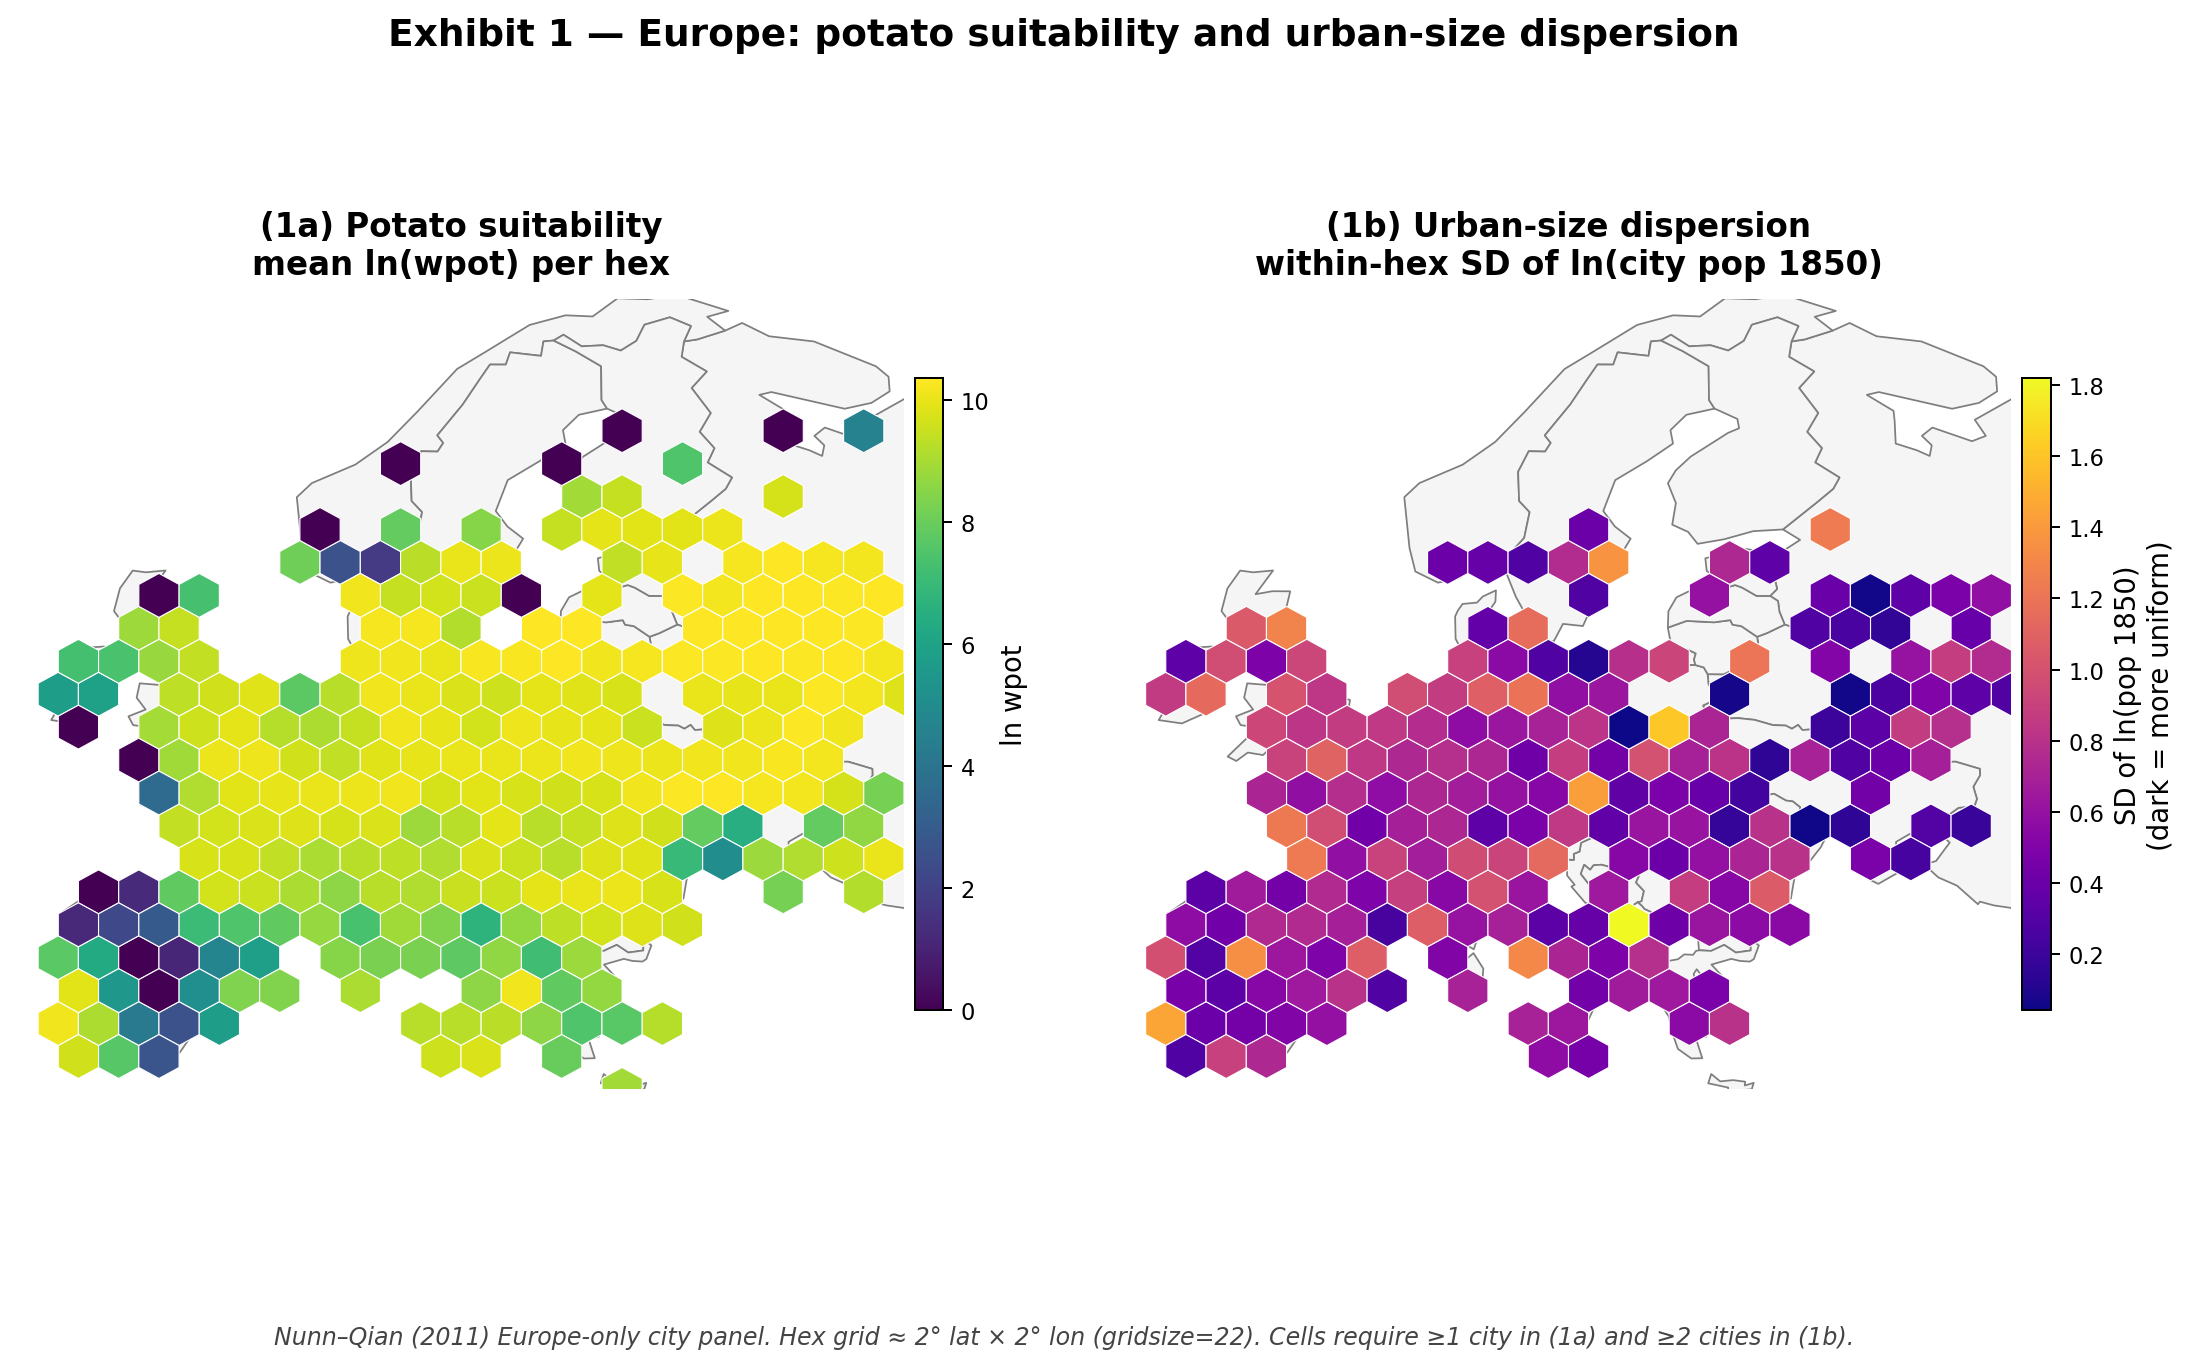
\includegraphics[width=0.95\linewidth]{exhibit1_europe.png}
\caption[Europe: potato suitability and income dispersion]%
{\textbf{Europe: potato suitability and income dispersion.}
Hex-binned heatmaps of the Nunn-Qian Europe-only city panel. Panel 1a colors each hex by the mean of potato suitability across cities in the cell; brighter cells indicate higher potato suitability. Panel 1b colors each hex by the within-hex standard deviation of $\ln$(city pop 1850), the income-dispersion measure used as the regional analysis outcome; darker cells indicate lower dispersion, i.e., a more uniform local income distribution. Hex grid is approximately $2^{\circ}$ latitude by $2^{\circ}$ longitude. Cells require at least one city in 1a and at least two in 1b.}
\label{fig:europe_exhibit}
\end{figure}

\begin{figure}[H]\centering
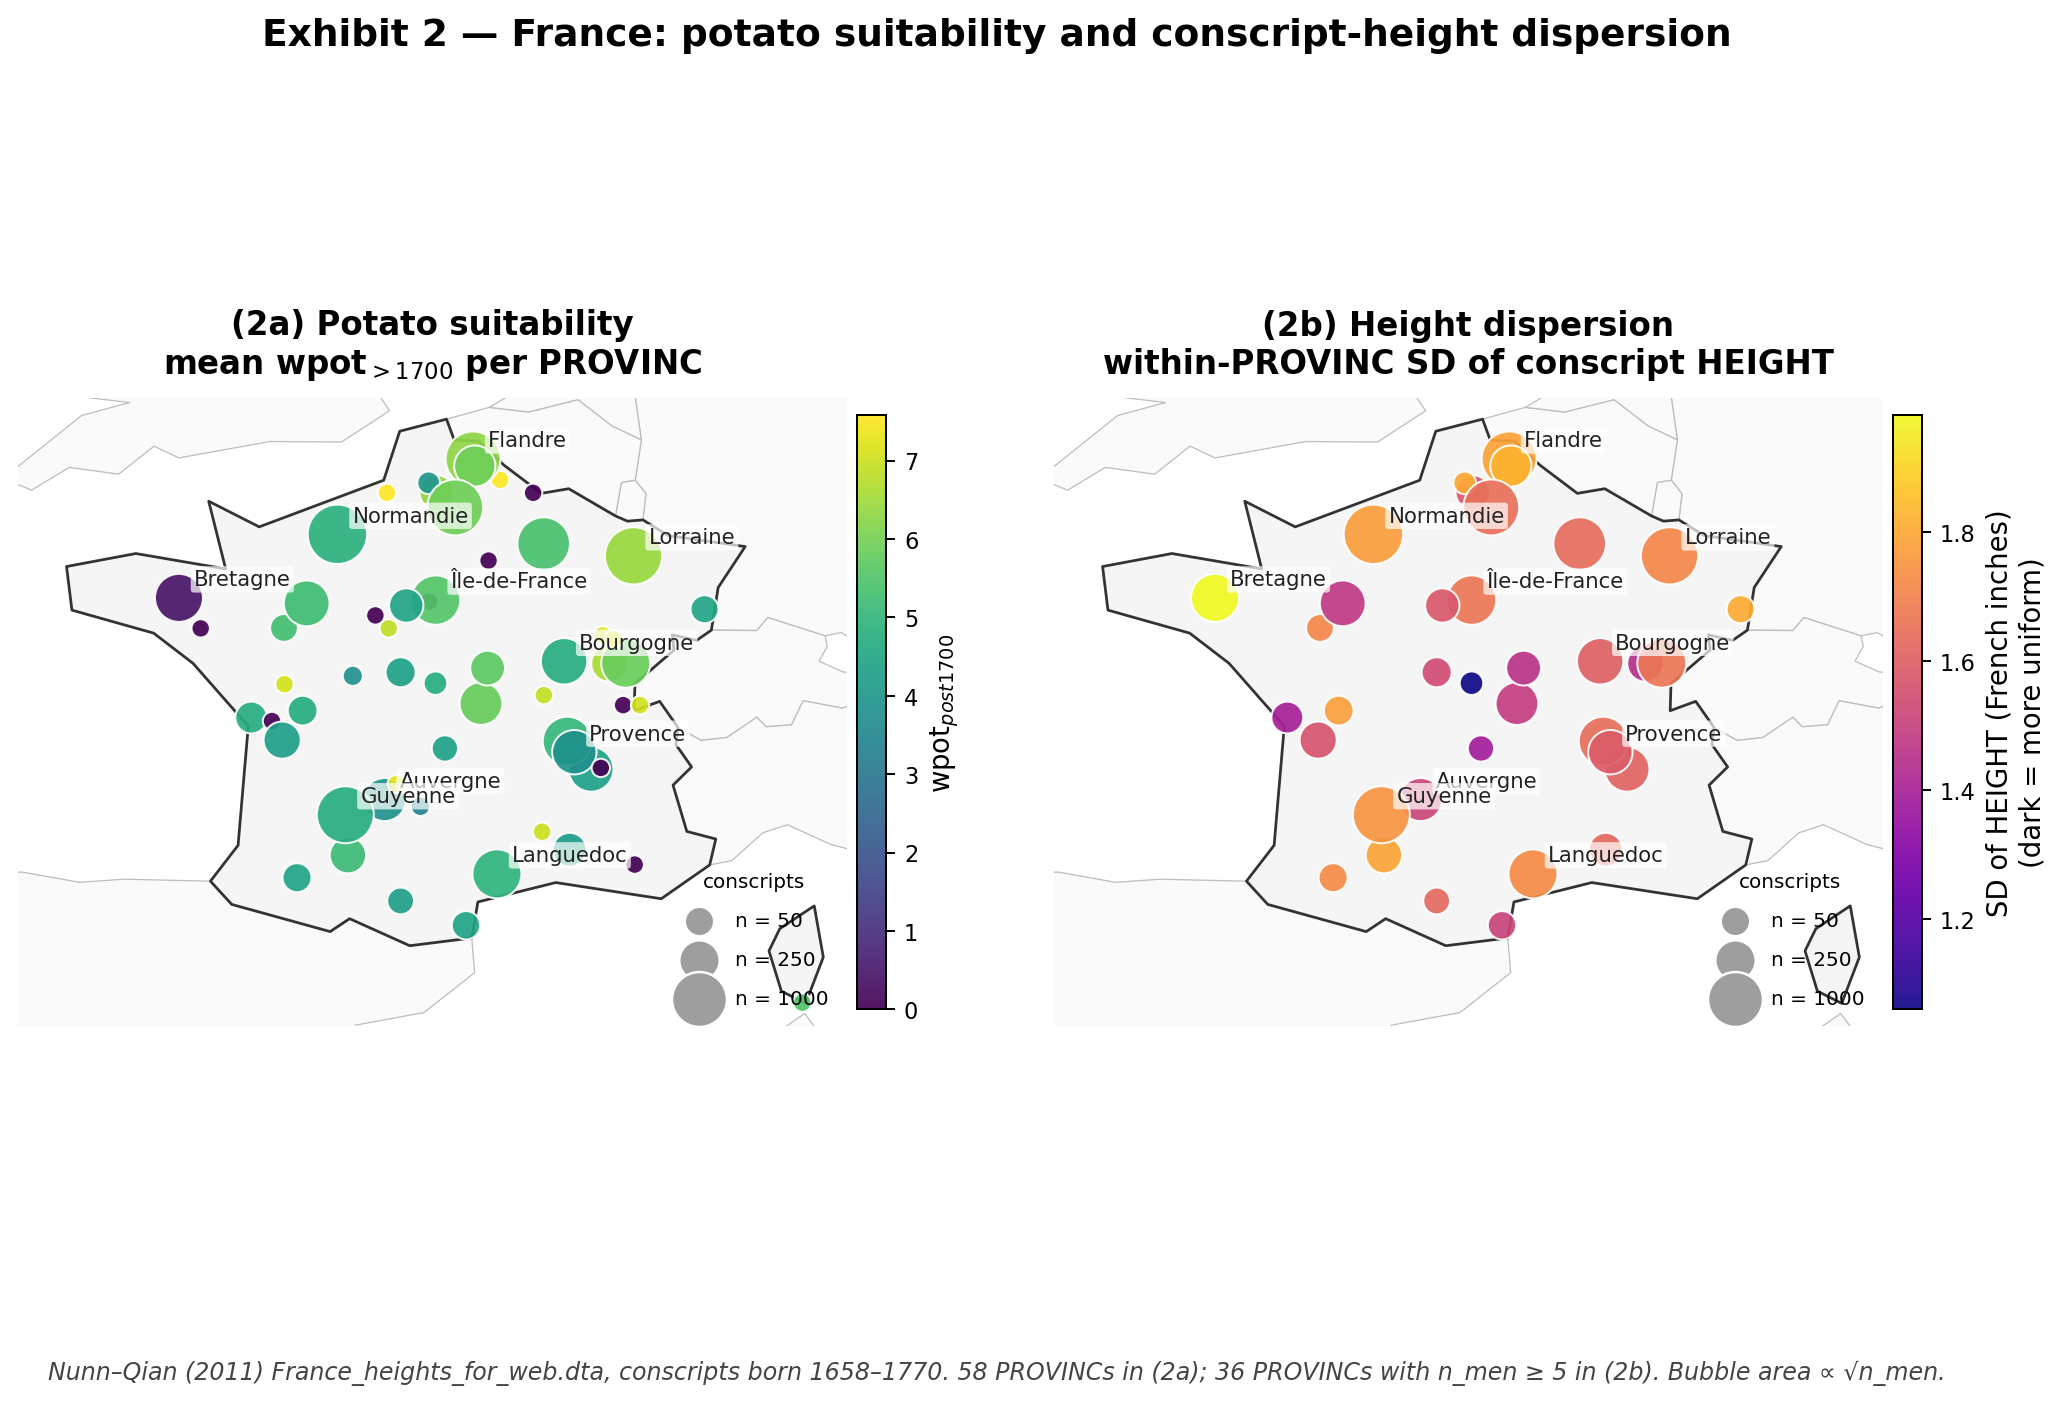
\includegraphics[width=0.95\linewidth]{exhibit2_france.png}
\caption[France: potato suitability and conscript-height dispersion]%
{\textbf{France: potato suitability and conscript-height dispersion.}
Each département is plotted at its conscript-weighted centroid; bubble area is proportional to the square root of the number of conscripts. Panel 2a colors bubbles by the département mean of the Nunn-Qian post-1700 potato suitability index. Panel 2b restricts to départements with at least five conscripts and colors bubbles by the within-département standard deviation of conscript heights; darker bubbles indicate lower dispersion. Selected major départements are labeled in both panels.}
\label{fig:france_exhibit}
\end{figure}

\FloatBarrier

% ---------------------------------
%  OUTCOMES
% ---------------------------------
\section{Outcomes}
I begin with a high-level summary in Table~\ref{tab:summary}, reporting the potato-suitability coefficient under the preferred specification for each outcome. Subsequent subsections present the full specification ladder for the EVS/WVS outcomes (Section~\ref{sec:wvs}), and the Nunn-Qian-derived outcomes (Section~\ref{sec:nq}).

\begin{table}[H]\centering
\caption{Summary of main results: preferred specification, by outcome}
\label{tab:summary}
\small
\begin{threeparttable}
\begin{tabular}{lcccccl}
\toprule
Outcome & $\hat\beta_{\ln\mathrm{wpot}}$ & SE & $p$ & $R^2$ & $N$ & Specification \\
\midrule
Communal-individual belief index           & $+0.0058^{**}$  & $(0.0025)$ & $0.027$ & $0.868$ & 98     & NUTS-1, cFE $+\,\ln$ oworld \\
Communal-individual belief index           & $+0.0047^{*}$   & $(0.0024)$ & $0.061$ & $0.744$ & 216    & NUTS-2, cFE $+$ full geog \\
Civic engagement (membership share)         & $-0.0017$       & $(0.0037)$ & $0.651$ & $0.795$ & 216    & NUTS-2, cFE $+$ full geog \\
Income dispersion: SD $\ln$(pop 1850)       & $-0.0498^{***}$ & $(0.0149)$ & $0.003$ & $0.209$ & 179    & NUTS-2, cFE $+$ full geog \\
France height: within-département SD        & $-0.0816^{***}$ & $(0.0225)$ & $0.001$ & $0.167$ & 36     & département level, $+$ ow\_idx \\
\bottomrule
\end{tabular}
\begin{tablenotes}\footnotesize
\item Each row reports the potato-suitability coefficient under the preferred specification for that outcome. Regional outcomes cluster SEs by country. $^{*}$~$p<.10$, $^{**}$~$p<.05$, $^{***}$~$p<.01$.
\end{tablenotes}
\end{threeparttable}
\end{table}

\FloatBarrier

% --- 3.1 WVS OUTCOMES ---
\subsection{World Values Survey Outcomes}\label{sec:wvs}
\paragraph{Communal-individual belief index.} I first describe effects on contemporary communalism in beliefs, as reported in Table~\ref{tab:communal}. Across the board, variation in potato suitability is a robust positive predictor of the communal-vs-individual belief index. At NUTS-1, the preferred specification gives $\hat\beta = 0.0058$, $p = 0.027$. The effect survives the addition of a control on old-world crop suitability and replicates at NUTS-2, with the most demanding specification giving $\hat\beta = 0.0047$, $p = 0.037$. The pooled cross-section without fixed effects also delivers a statistically significant positive coefficient at NUTS-2 ($\hat\beta = 0.008$, $p = 0.010$). Figure~\ref{fig:exhibit_communal} visualizes the positive relationship, while also elucidating the absence of outliers skewing this trend; the upward-sloping fitted line confirms that the headline result is not driven by extreme observations.

\paragraph{Magnitude.} A one-within-country-SD increase in potato suitability shifts the communal-index by approximately $0.20\sigma$ within the given country and $0.08\sigma$ in the overall distribution.

\begin{table}[H]\centering
\caption{Potato suitability and the communal-individual belief index}
\label{tab:communal}
\small
\begin{threeparttable}
\begin{tabular}{l*{6}{c}}
\toprule
 & \multicolumn{3}{c}{Pooled OLS} & \multicolumn{3}{c}{Country fixed effects} \\
\cmidrule(lr){2-4}\cmidrule(lr){5-7}
 & (1) & (2) & (3) & (A) & \textbf{(B)} & (C) \\
\midrule
\multicolumn{7}{l}{\emph{Panel A. NUTS-1 (regions)}} \\
$\ln$ wpot & $+0.0028$ & $+0.0002$ & $+0.0071^{**}$ & $+0.0049^{***}$ & $\mathbf{+0.0058^{**}}$ & $+0.0046$ \\
           & $(0.0018)$ & $(0.0028)$ & $(0.0033)$ & $(0.0017)$ & $\mathbf{(0.0025)}$ & $(0.0034)$ \\
$R^2$ & $0.011$ & $0.025$ & $0.336$ & $0.866$ & $0.868$ & $0.872$ \\
$N$   & $98$ & $98$ & $98$ & $98$ & $98$ & $98$ \\
\addlinespace
\multicolumn{7}{l}{\emph{Panel B. NUTS-2 (regions)}} \\
$\ln$ wpot & $+0.0035^{*}$ & $+0.0014$ & $+0.0080^{***}$ & $+0.0024$ & $\mathbf{+0.0055^{**}}$ & $+0.0047^{*}$ \\
           & $(0.0021)$ & $(0.0028)$ & $(0.0029)$ & $(0.0028)$ & $\mathbf{(0.0026)}$ & $(0.0024)$ \\
$R^2$ & $0.012$ & $0.018$ & $0.263$ & $0.734$ & $0.740$ & $0.744$ \\
$N$   & $216$ & $216$ & $216$ & $216$ & $216$ & $216$ \\
\midrule
$\ln$ oworld          &   & \checkmark & \checkmark &   & \checkmark & \checkmark \\
Other geog controls   &   &            & \checkmark &   &            & \checkmark \\
Country FE            &   &            &            & \checkmark & \checkmark & \checkmark \\
\bottomrule
\end{tabular}
\begin{tablenotes}\footnotesize
\item Robust SEs in parentheses; cFE columns use SEs clustered by country. Other geog controls $=$ $\ln$ elevation, $\ln$ tropics, $\ln$ rugged. The preferred main column is in \textbf{bold}. $^{*}$ $p<.10$, $^{**}$ $p<.05$, $^{***}$ $p<.01$.
\end{tablenotes}
\end{threeparttable}
\end{table}

\begin{figure}[H]\centering
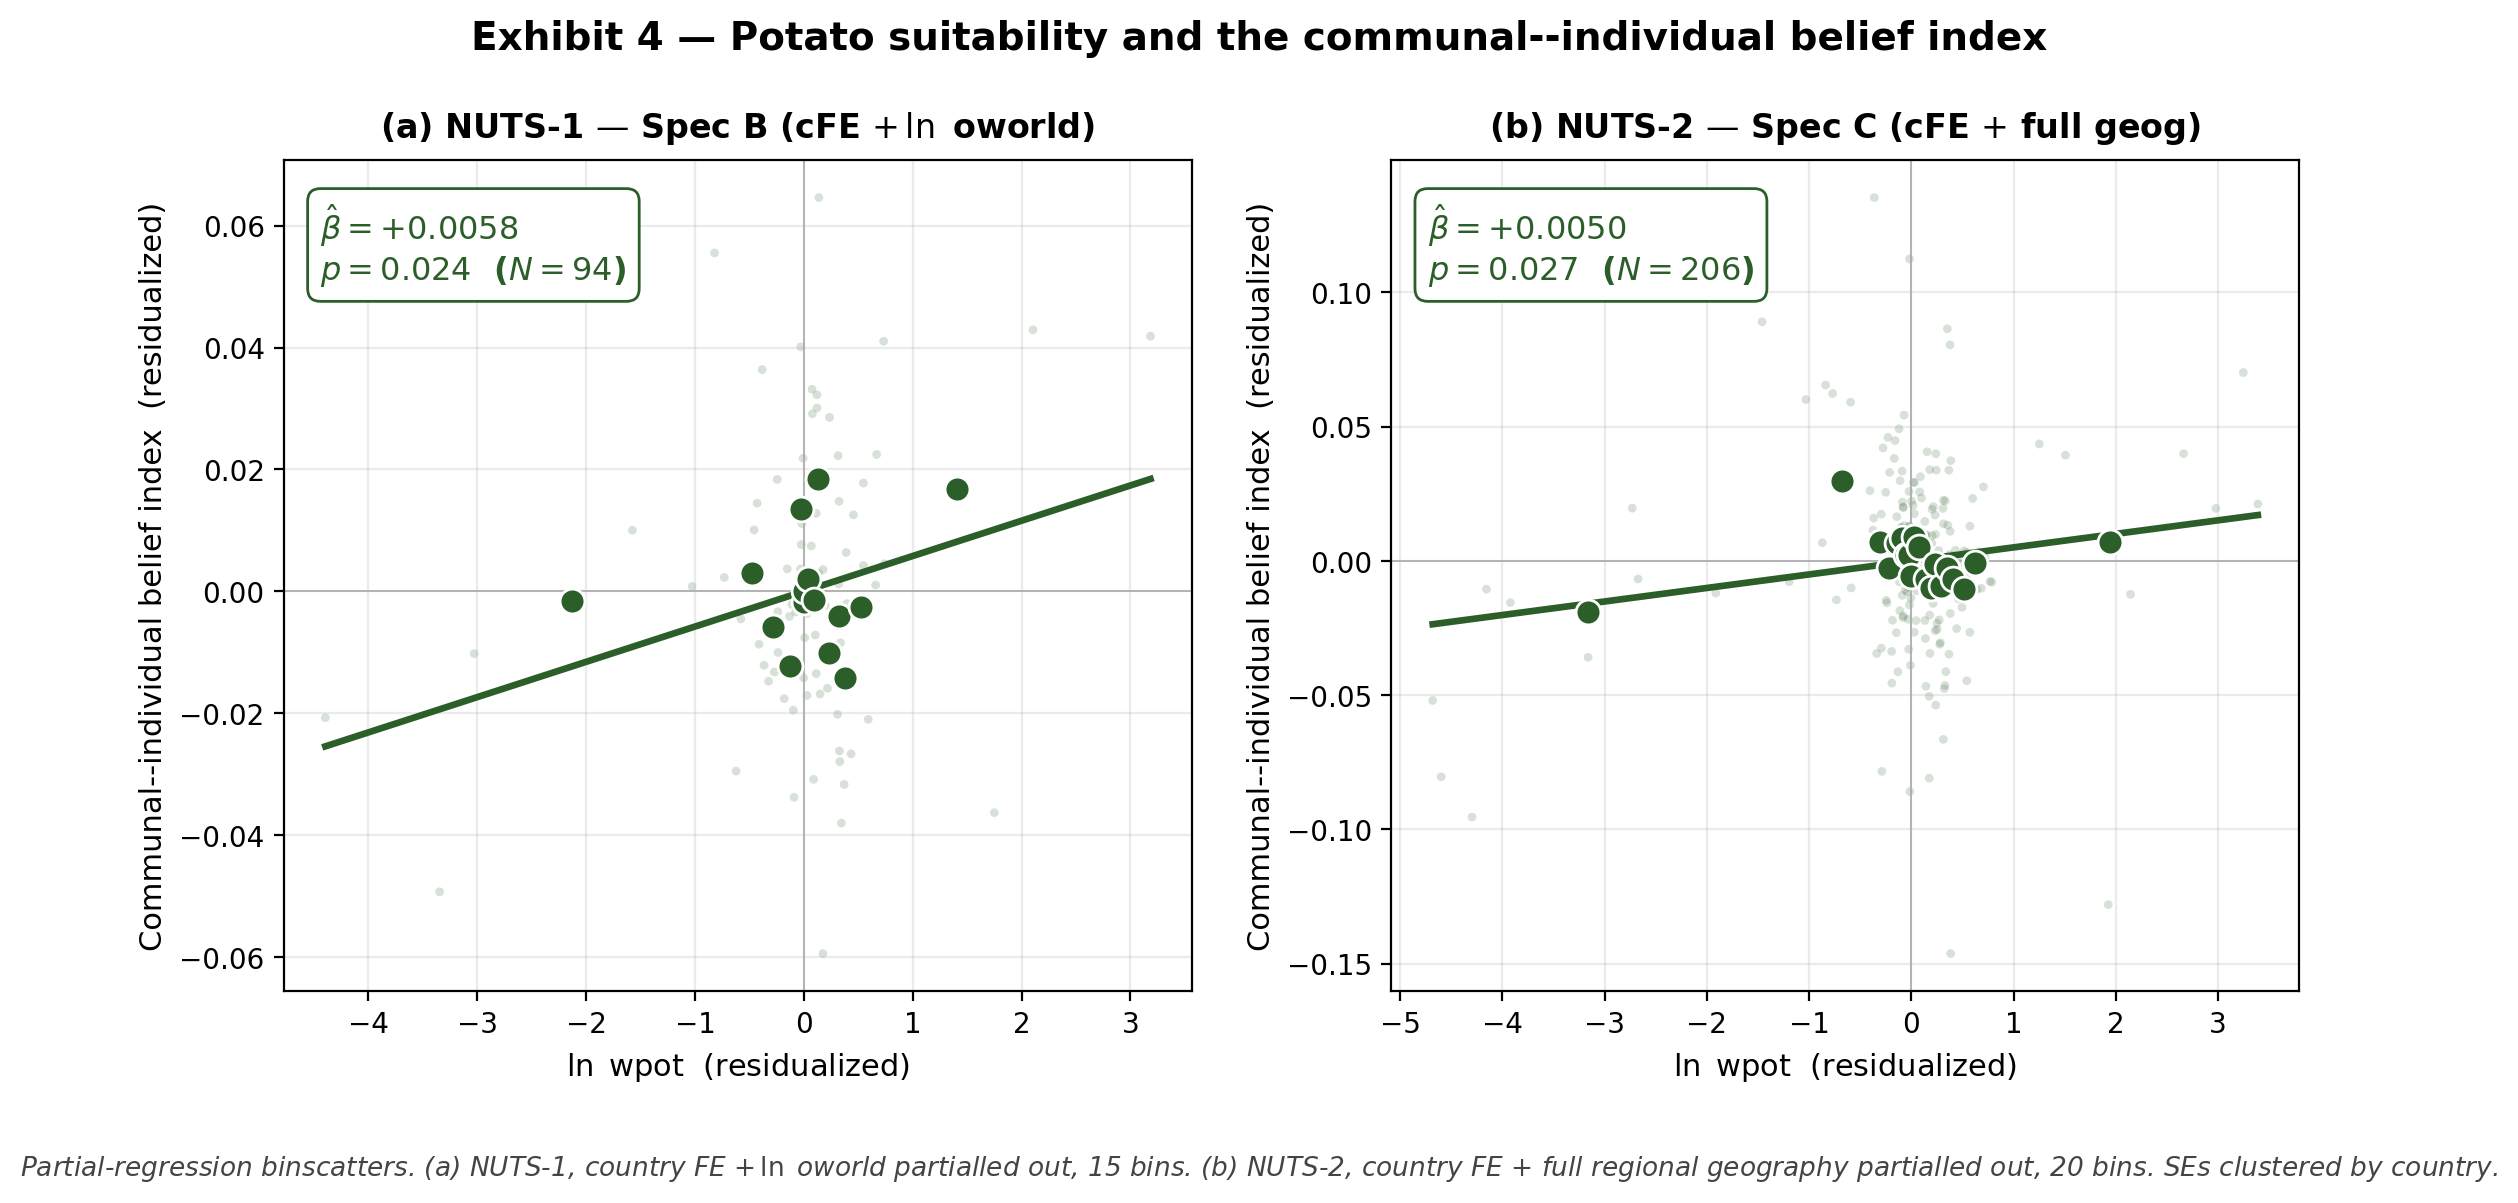
\includegraphics[width=0.95\linewidth]{exhibit4_communal.png}
\caption[Communal-individual belief index: partial-regression binscatter]%
{\textbf{Communal-individual belief index: partial-regression binscatter.} Panel a: NUTS-1, country fixed effects and old-world crop suitability partialled out. Panel b: NUTS-2, country fixed effects and the full regional geography partialled out. Twenty equal-frequency bin means, the filled markers, are overlaid on the underlying residuals, the faint markers, with the OLS fit. The boxed $\hat\beta$ and $p$-value in each panel correspond to the regression coefficient in Table~\ref{tab:communal}.}
\label{fig:exhibit_communal}
\end{figure}

\FloatBarrier

\paragraph{Civic engagement.} Civic-engagement results are reported in Table~\ref{tab:civic}. Under the preferred within-country specification, potato suitability does not predict the share of voluntary organizations a respondent reports belonging to: $\hat\beta = 0.0006$ at NUTS-1 under the preferred specification, $p = 0.870$, and $\hat\beta = -0.0017$ at NUTS-2 under the most demanding specification, $p = 0.651$. The pooled cross-section does deliver a positive significant coefficient at both NUTS levels once old-world crop suitability is added, with $\hat\beta = 0.006$, $p = 0.001$ at NUTS-2, but this is the same cross-country east-west gradient that absorbs the bivariate communal-index signal. Within country, organizational membership is essentially uncorrelated with potato suitability. The partial-regression binscatter is shown in Figure~\ref{fig:exhibit_civic}.

\begin{table}[H]\centering
\caption{Potato suitability and civic engagement (membership share)}
\label{tab:civic}
\small
\begin{threeparttable}
\begin{tabular}{l*{6}{c}}
\toprule
 & \multicolumn{3}{c}{Pooled OLS} & \multicolumn{3}{c}{Country fixed effects} \\
\cmidrule(lr){2-4}\cmidrule(lr){5-7}
 & (1) & (2) & (3) & (A) & (B) & \textbf{(C)} \\
\midrule
\multicolumn{7}{l}{\emph{Panel A. NUTS-1 (regions)}} \\
$\ln$ wpot & $+0.0040^{*}$  & $+0.0075^{***}$ & $-0.0004$ & $+0.0010$ & $+0.0006$ & $\mathbf{+0.0011}$ \\
           & $(0.0022)$ & $(0.0026)$ & $(0.0029)$ & $(0.0041)$ & $(0.0037)$ & $\mathbf{(0.0031)}$ \\
$R^2$ & $0.020$ & $0.042$ & $0.203$ & $0.870$ & $0.871$ & $0.878$ \\
$N$   & $98$ & $98$ & $98$ & $98$ & $98$ & $98$ \\
\addlinespace
\multicolumn{7}{l}{\emph{Panel B. NUTS-2 (regions)}} \\
$\ln$ wpot & $+0.0012$ & $+0.0061^{***}$ & $-0.0039^{**}$ & $-0.0016$ & $-0.0017$ & $\mathbf{-0.0017}$ \\
           & $(0.0021)$ & $(0.0019)$ & $(0.0019)$ & $(0.0040)$ & $(0.0035)$ & $\mathbf{(0.0037)}$ \\
$R^2$ & $0.002$ & $0.046$ & $0.275$ & $0.792$ & $0.792$ & $0.795$ \\
$N$   & $216$ & $216$ & $216$ & $216$ & $216$ & $216$ \\
\midrule
$\ln$ oworld          &   & \checkmark & \checkmark &   & \checkmark & \checkmark \\
Other geog controls   &   &            & \checkmark &   &            & \checkmark \\
Country FE            &   &            &            & \checkmark & \checkmark & \checkmark \\
\bottomrule
\end{tabular}
\begin{tablenotes}\footnotesize
\item Robust SEs in parentheses; cFE columns use SEs clustered by country. Other geog controls $=$ $\ln$ elevation, $\ln$ tropics, $\ln$ rugged. The preferred main column is in \textbf{bold}. $^{*}$ $p<.10$, $^{**}$ $p<.05$, $^{***}$ $p<.01$.
\end{tablenotes}
\end{threeparttable}
\end{table}

\begin{figure}[H]\centering
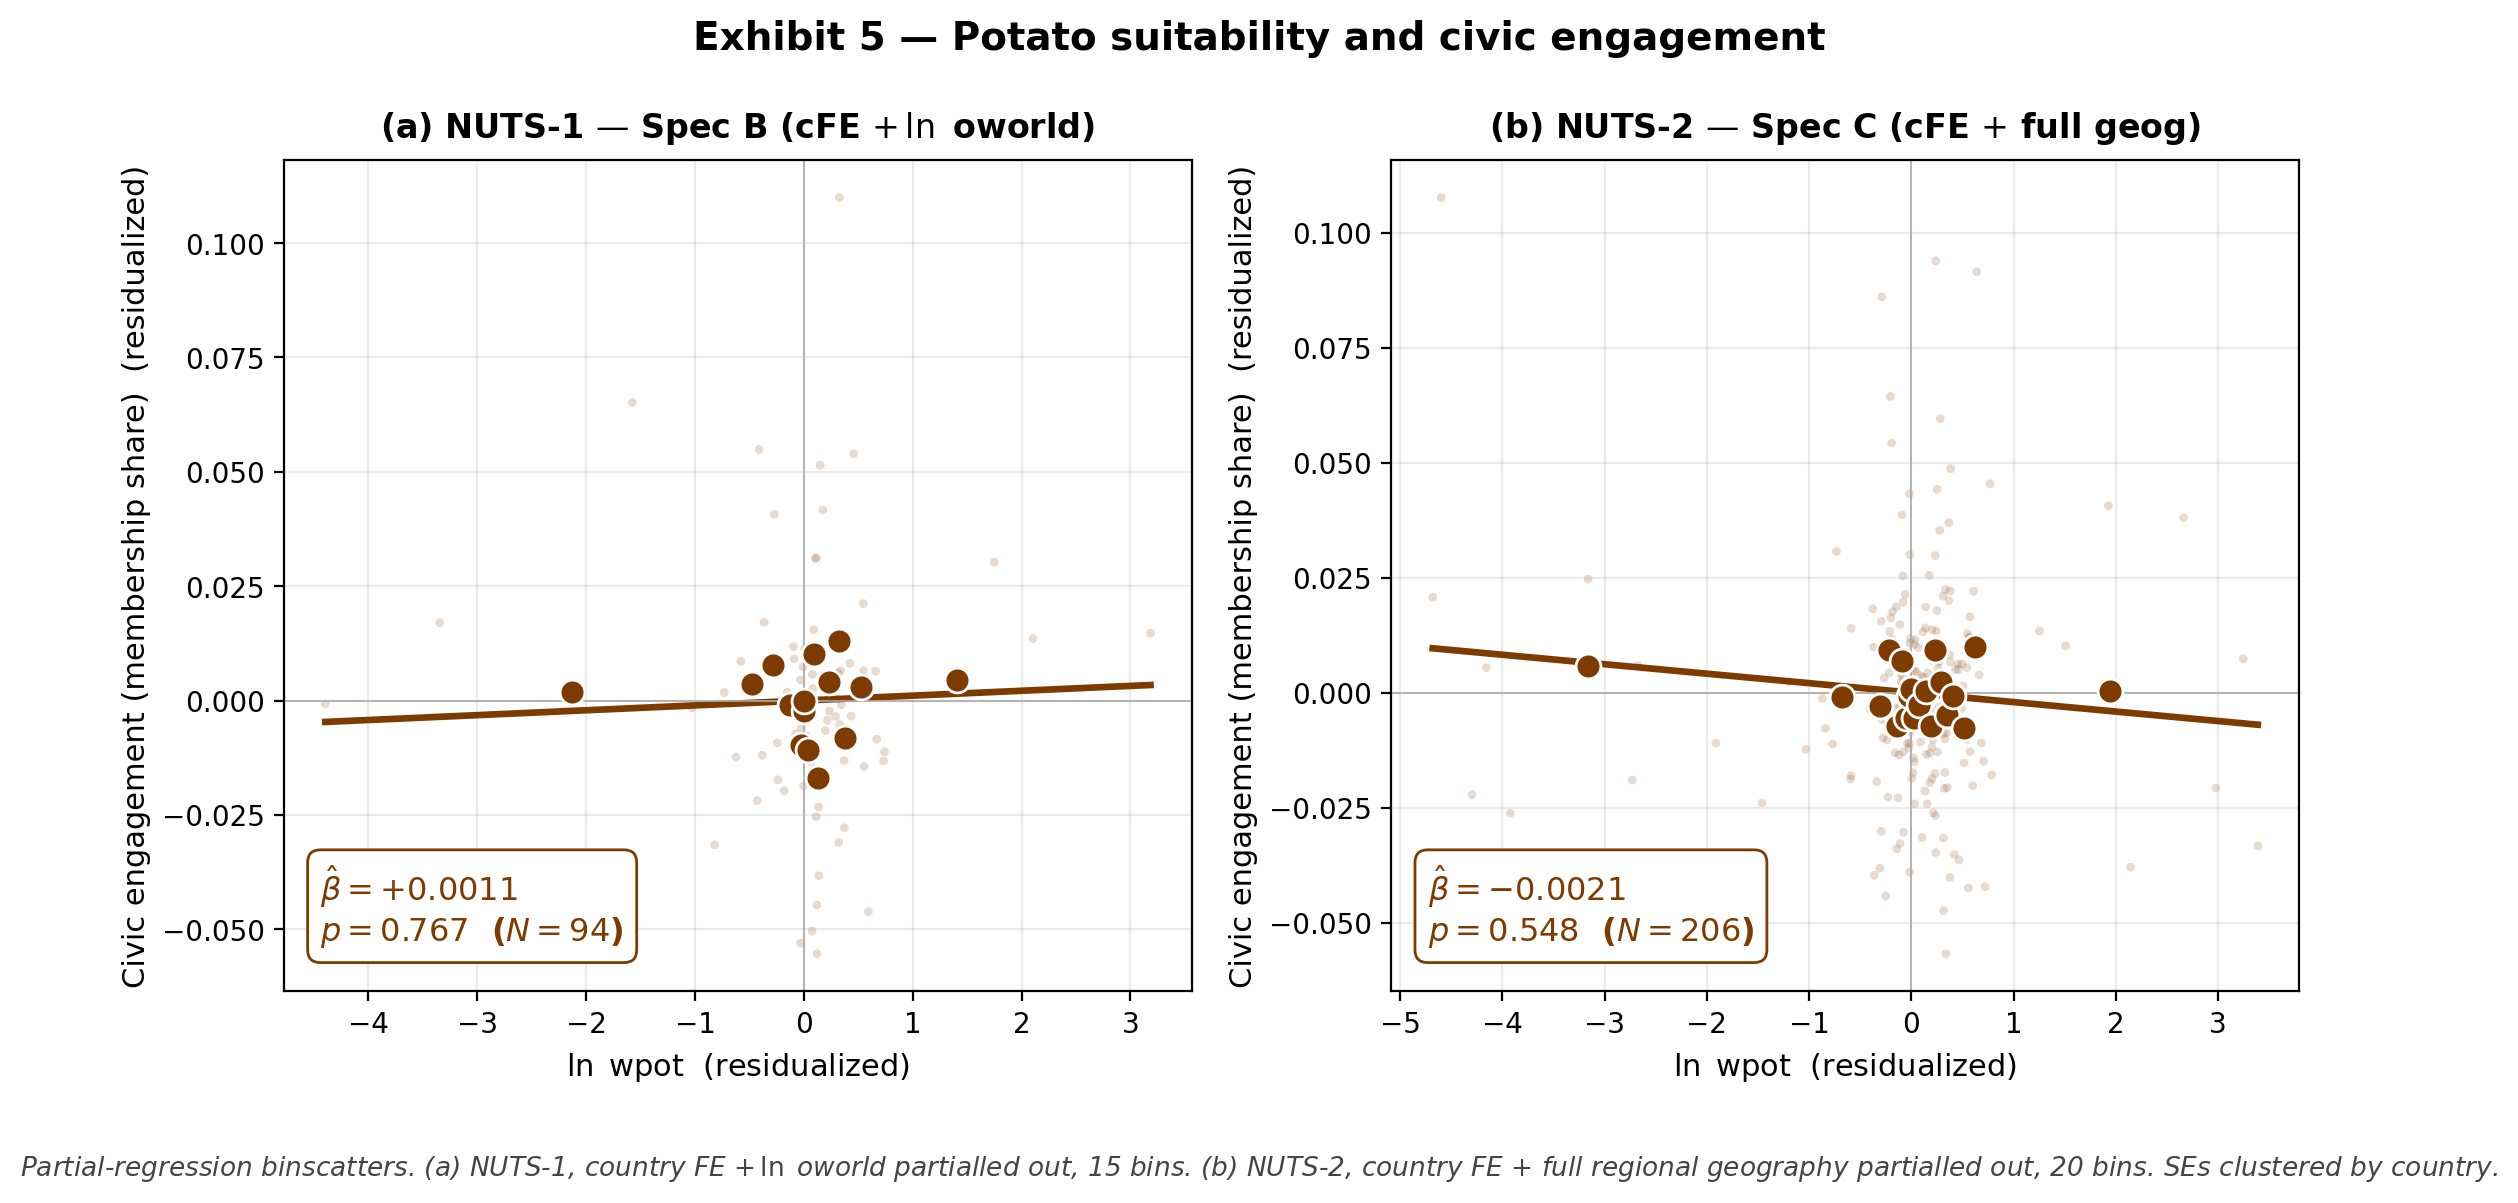
\includegraphics[width=0.95\linewidth]{exhibit5_civic.png}
\caption[Civic engagement: partial-regression binscatter]%
{\textbf{Civic engagement: partial-regression binscatter.} Panel a: NUTS-1, country fixed effects and old-world crop suitability partialled out. Panel b: NUTS-2, country fixed effects and the full regional geography partialled out. The fitted line is essentially flat at both levels, confirming the null result reported in Table~\ref{tab:civic}.}
\label{fig:exhibit_civic}
\end{figure}

\FloatBarrier

% --- 3.3 NUNN-QIAN OUTCOMES ---
\subsection{Nunn-Qian Outcomes}\label{sec:nq}
I now report one outcome derived from the Nunn-Qian historical city panel, income dispersion, and one outcome derived from the France conscript-height microdata, within-département height dispersion.

\paragraph{Income dispersion.} Table~\ref{tab:pop_sd} reports the regressions on standard deviation of incomes, the headline result of this paper. Under country fixed effects, the within-country potato effect on income dispersion is strongly negative and survives the most demanding specification: at NUTS-2 it gives $\hat\beta = -0.0498$, $p = 0.003$, $R^2 = 0.21$. Defining geographic units at the NUTS-1 also produces a negative coefficient, $\hat\beta = -0.049$, $p = 0.092$, though with weaker power. A unit increase in potato suitability at NUTS-2 lowers dispersion in urbanization by approximately $0.16\sigma$ in the overall distribution. Following the example of \citet{NunnQian2011}, we can reasonably assume urbanization to be a reliable proxy for income within this context. In sum, within a given country, regions with higher potato suitability had a more uniform income distribution relative to their grain-advantaged counterparts. Figure~\ref{fig:binscatter}, panel a, gives the corresponding partial-regression binscatter.

\begin{table}[H]\centering
\caption{Potato suitability and income dispersion: SD $\ln$(city pop 1850)}
\label{tab:pop_sd}
\small
\begin{threeparttable}
\begin{tabular}{l*{6}{c}}
\toprule
 & \multicolumn{3}{c}{Pooled OLS} & \multicolumn{3}{c}{Country fixed effects} \\
\cmidrule(lr){2-4}\cmidrule(lr){5-7}
 & (1) & (2) & (3) & (A) & (B) & \textbf{(C)} \\
\midrule
\multicolumn{7}{l}{\emph{Panel A. NUTS-1 (regions)}} \\
$\ln$ wpot & $-0.0008$ & $-0.0126$ & $-0.0041$ & $-0.0271$ & $-0.0431^{*}$ & $\mathbf{-0.0491^{*}}$ \\
           & $(0.0188)$ & $(0.0249)$ & $(0.0268)$ & $(0.0266)$ & $(0.0243)$ & $\mathbf{(0.0281)}$ \\
$R^2$ & $0.000$ & $0.009$ & $0.027$ & $0.188$ & $0.212$ & $0.269$ \\
$N$   & $96$ & $96$ & $96$ & $96$ & $96$ & $96$ \\
\addlinespace
\multicolumn{7}{l}{\emph{Panel B. NUTS-2 (regions)}} \\
$\ln$ wpot & $-0.0071$ & $-0.0263$ & $-0.0312$ & $-0.0106$ & $-0.0388^{**}$ & $\mathbf{-0.0498^{***}}$ \\
           & $(0.0140)$ & $(0.0165)$ & $(0.0199)$ & $(0.0249)$ & $(0.0171)$ & $\mathbf{(0.0149)}$ \\
$R^2$ & $0.002$ & $0.020$ & $0.027$ & $0.171$ & $0.195$ & $0.209$ \\
$N$   & $179$ & $179$ & $179$ & $179$ & $179$ & $179$ \\
\midrule
$\ln$ oworld          &   & \checkmark & \checkmark &   & \checkmark & \checkmark \\
Other geog controls   &   &            & \checkmark &   &            & \checkmark \\
Country FE            &   &            &            & \checkmark & \checkmark & \checkmark \\
\bottomrule
\end{tabular}
\begin{tablenotes}\footnotesize
\item Outcome: within-region SD of $\ln$(city pop 1850), the income-dispersion proxy following \citet{NunnQian2011}. Robust SEs in parentheses; cFE columns use SEs clustered by country. Other geog controls $=$ $\ln$ elevation, $\ln$ tropics, $\ln$ rugged. The preferred main column is in \textbf{bold}. $^{*}$ $p<.10$, $^{**}$ $p<.05$, $^{***}$ $p<.01$.
\end{tablenotes}
\end{threeparttable}
\end{table}

\FloatBarrier

\paragraph{Conscript-height dispersion in France.} Table~\ref{tab:fr_height_sd} reports the regional standard deviation of height regressions. The bivariate effect is null, but once the index for old-world crop suitability is added, the coefficient on potato suitability becomes strongly negative: $\hat\beta = -0.0816$, $p = 0.001$, $R^2 = 0.17$ in the preferred specification. The specification that adds the full geography indices retains the sign and statistical significance, $\hat\beta = -0.0669$, $p = 0.010$. The bivariate baseline and the all-controls specification are null, however: the bivariate baseline because the cross-département variation in potato suitability is dominated by other ecological gradients, and the all-controls specification because it over-parameterizes a sample of $N = 36$ départements. The cross-département SD of the dependent variable is approximately $0.18$, so $\hat\beta = -0.082$ implies a roughly $0.4\sigma$ effect under the preferred specification. The direction parallels the result on degree of income inequality: within France, départements with higher potato suitability had a more uniform distribution of conscript heights, indicating a smaller spread in physical welfare across the working-age male population. Figure~\ref{fig:binscatter}, panel b, gives the corresponding partial-regression scatter.

\begin{table}[H]\centering
\caption{Potato suitability and within-département SD of conscript heights in France}
\label{tab:fr_height_sd}
\small
\begin{threeparttable}
\begin{tabular}{l*{4}{c}}
\toprule
 & (1) & \textbf{(2)} & (3) & (4) \\
 & Bivariate & \textbf{$+\,\mathrm{idx}_{\text{ow}}$} & $+$ full geog & $+$ all controls \\
\midrule
$\mathrm{wpot}^{>1700}$ & $-0.0310$ & $\mathbf{-0.0816^{***}}$ & $-0.0669^{***}$ & $-0.0370$ \\
                       & $(0.0287)$ & $\mathbf{(0.0225)}$ & $(0.0242)$ & $(0.0311)$ \\
$R^2$ & $0.041$ & $0.167$ & $0.210$ & $0.250$ \\
$N$   & $36$ & $36$ & $36$ & $36$ \\
\midrule
Old-world suitability index             &   & \checkmark & \checkmark & \checkmark \\
Other geog indices (rugged, elev, trop) &   &            & \checkmark & \checkmark \\
Lat / dist-coast / malaria indices      &   &            &            & \checkmark \\
\bottomrule
\end{tabular}
\begin{tablenotes}\footnotesize
\item Outcome: within-département SD of conscript height, computed across conscripts in each département with $n_{\text{men}} \geq 5$. Continuous decile-rank indices $\sum_d d\cdot \mathrm{dec}_d$ used in place of the full decile-dummy block because $N = 36$. HC1 robust SEs. The main column is in \textbf{bold}. $^{*}$ $p<.10$, $^{**}$ $p<.05$, $^{***}$ $p<.01$.
\end{tablenotes}
\end{threeparttable}
\end{table}

\begin{figure}[H]\centering
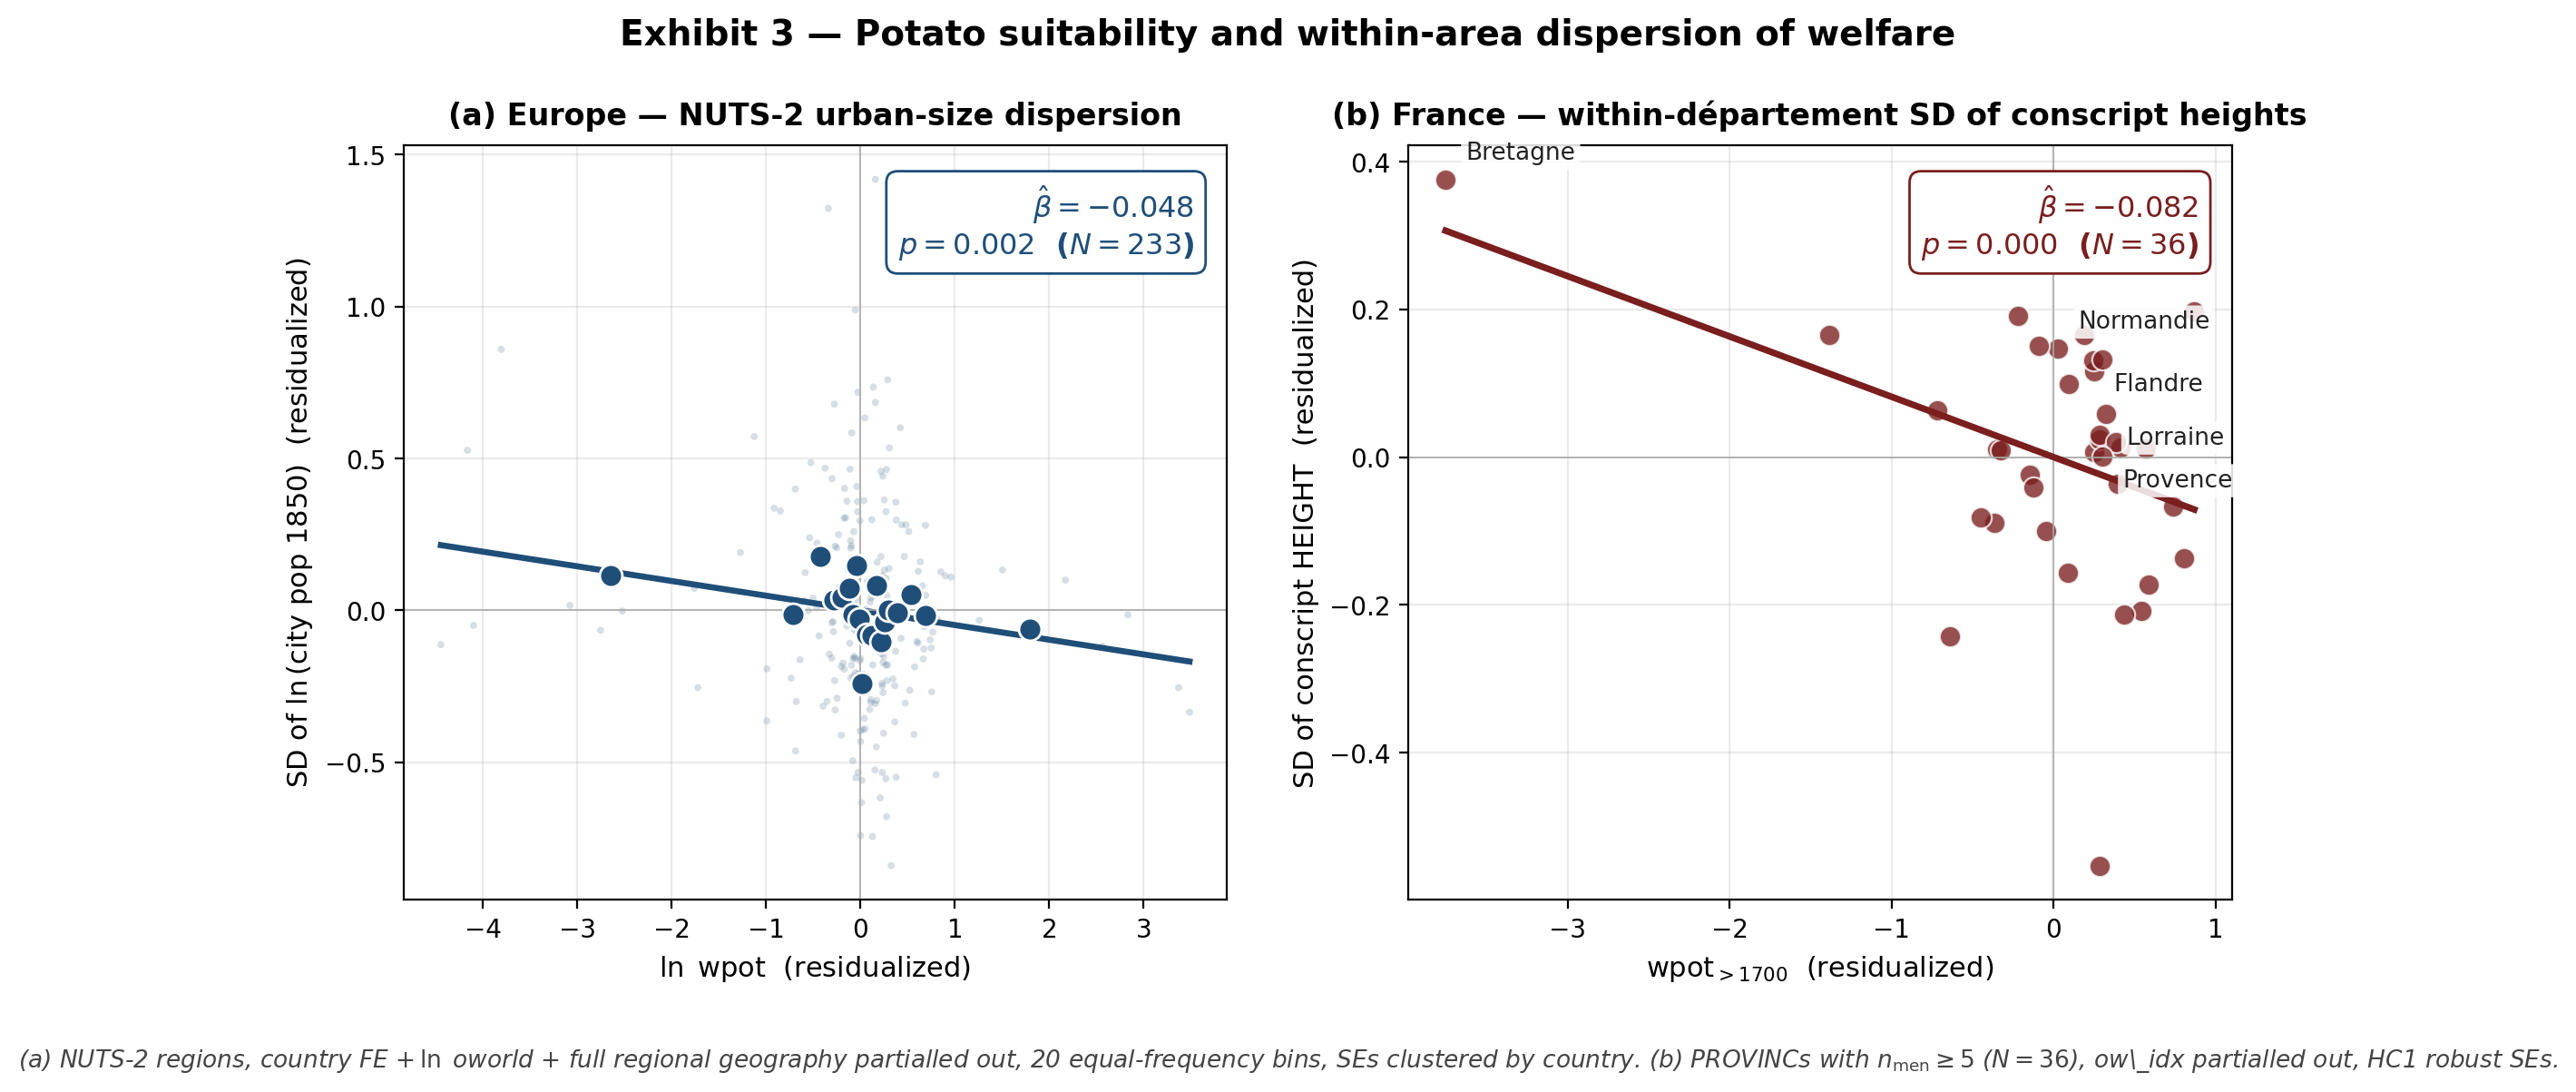
\includegraphics[width=0.95\linewidth]{exhibit3_binscatter.png}
\caption[Headline dispersion result: partial-regression binscatter]%
{\textbf{Headline dispersion result: partial-regression binscatter.} Panel a plots the residualized within-region standard deviation of $\ln$(city pop 1850) against residualized potato suitability at the NUTS-2 level, after partialling out country fixed effects, old-world crop suitability, and the remaining pre-treatment ecological controls; 20 equal-frequency bin means overlaid on the residuals, OLS fit. Panel b plots the residualized within-département standard deviation of conscript height against residualized potato suitability at the département level, $N = 36$, with the old-world-suitability index partialled out. The slopes correspond to the coefficients in Tables~\ref{tab:pop_sd} and~\ref{tab:fr_height_sd}.}
\label{fig:binscatter}
\end{figure}

\FloatBarrier

% ---------------------------------
%  CONCLUSION
% ---------------------------------
\section{Conclusion}
\subsection{Takeaways}
These results underlie three broader takeaways.

First of all, suitability for potato cultivation is associated with an increase in contemporary preferences for communitarian ideologies.

In particular, a one-within-country-SD increase in potato suitability raises the EVS/WVS communal-vs-individual belief index by approximately $0.20\sigma$, robust to conditioning on old-world crop suitability and replicates at the more granular NUTS-2 level of geographic aggregation.

Additionally, potato suitability strongly predicts lower dispersion in income and physical welfare. At NUTS-2 under the preferred FE specification, $\hat\beta = -0.050$, $p = 0.003$ on the within-region SD of $\ln$(city pop 1850); in France, $\hat\beta = -0.082$, $p = 0.001$ on the within-département SD of conscript heights. Both measures suggest that environments suitable for potato farming tend to support more equal distributions of income and consumption, proxied by urbanization and height. The former mirrors the prediction of \citet{NunnQian2011}'s argument that the potato supported a denser, more evenly distributed agricultural surplus; the height-dispersion result extends the same logic to a physical-welfare outcome at the individual level.

\textit{Third}, civic engagement appears uncorrelated with regional variation in potato suitability. Combined with a significant, positive relationship with communal beliefs, this suggests that the mechanism operates through values, such as preferences over redistribution and in-group orientation, without extending to observable behavioral shifts. Nevertheless, this finding relies upon self-reported organizational membership; extensions exploiting available historical data on union membership, church attendance, or political party involvement could alternately emphasize or call into question this null result.

\subsection{Mechanisms}
Three candidate channels are consistent with the documented pattern.

\textit{Nutritional density.} The potato is calorie-dense and provides a more complete nutritional profile per unit of land than other staple grains typical within the European diet. Higher potato suitability therefore raises the local subsistence floor, compressing the spread of consumption and thus promoting less disparity in economic and physical well-being

\textit{Appropriability.} Tubers are less visible during the growing process, heavier, and perishable once removed from the soil. Consequently, relative to cereals, they are harder to monitor, store, transport, and tax \citep{MaysharMoavPascali2022}. Higher potato suitability therefore tends to undermine the development of extractive hierarchies. Thus, potato cultivation renders taxation less efficient, impeding the concentration of economic and political power.

\textit{Horticulture-versus-agriculture scale.} Potato cultivation is viable at household scale, while cereal cultivation favors larger estates, equipped with a larger, more specialized labor force and agricultural technology \citep{AlesinaGiulianoNunn2013}. A potato-suitable region is therefore more likely to sustain a network of self-sustaining households and small land-holders rather than a hierarchy concentrated around a few large producers. This mechanism clarifies the link between suitability for potato cultivation and communalism beliefs, since the resultant economic structure would necessarily strengthen kin ties relative to ties to the broader social network.

\subsection{Extensions}
Several extensions could strengthen the depth and breadth of this analysis. First of all, I could examine additional historical microdata in the studied regions, such as estate records, tax records, and child mortality records, to further examine trends in wealth, income, and well-being, respectively. Additionally, this paper would be strengthened by a stronger integration of political economy. I omit description of the tax structures which developed in the studied countries; further analysis could examine the link between potato cultivation and features of the tax system, such as efficiency or progressivity. Moreover, I am interested in how economic historians typically proxy for ideology and values within the historical context. My results on contemporary communalism could be strengthened by analysis of ideological variation more proximate to the shock. In this vein, I would be interested in how potato variation correlates with attendance and membership in religious institutions, unions, and political parties, a direct measure of civic engagement and reasonable proxy for values. Such extensions could assist in better identifying the relative potency of and interplay between each of the suggested mechanisms. Nevertheless, this analysis thus far succeeds in identifying a potential contributing factor to the divergence in economic development and ideology in Europe in the modern age, suggesting that the ``Potato Europe'' boundary drawn by Tsetov's comical map may be more salient than he could have ever imagined.

% ---------------------------------
%  BIBLIOGRAPHY
% ---------------------------------
\clearpage
\bibliographystyle{apalike}
\bibliography{biblio}

% ---------------------------------
%  APPENDIX
% ---------------------------------
% potato_appendix.tex --- Appendix to drop into the paper.
% Required preamble (already in main paper): booktabs, threeparttable,
% amsmath, amssymb, array, placeins (for \FloatBarrier).
% Use \appendix before \input{}.

\appendix
\section{Survey items used in the EVS5/WVS7 Joint v5}
\label{app:items}

This appendix lists the 22 EVS/WVS items used in constructing the two
respondent-level outcomes. All response codes are taken from the EVS/WVS Joint
v5 codebook; negative codes (no answer, don't know, item not in country's
questionnaire) are coded as missing throughout. The respondent-level communal
index is the simple mean of the 11 rescaled items in Table~\ref{tab:items_communal};
the civic engagement share is the proportion of the 11 organization types in
Table~\ref{tab:items_civic} for which the respondent reports membership, conditional
on at least six items being answered.

\begin{table}[!htbp]\centering
\caption{Items used in the communal--individual belief index}
\label{tab:items_communal}
\footnotesize
\begin{threeparttable}
\begin{tabular}{p{0.9cm} p{4.3cm} p{1.0cm} p{5.0cm} p{3.2cm}}
\toprule
Code & Label & Scale & Original response scale & Rescaling to $[0,1]$ \\
\midrule
C038 & People who don't work turn lazy & 5-point & 1 = Agree strongly $\dots$ 5 = Disagree strongly & $(5-x)/4$; agree $=$ communal \\
C039 & Work is a duty towards society & 5-point & 1 = Agree strongly $\dots$ 5 = Disagree strongly & $(5-x)/4$; agree $=$ communal \\
C041 & Work should come first even if it means less spare time & 5-point & 1 = Agree strongly $\dots$ 5 = Disagree strongly & $(5-x)/4$; agree $=$ communal \\
D026\_03 & Duty towards society to have children & 5-point & 1 = Agree strongly $\dots$ 5 = Disagree strongly & $(5-x)/4$; agree $=$ communal \\
D026\_05 & It is childs duty to take care of ill parent & 5-point & 1 = Agree strongly $\dots$ 5 = Disagree strongly & $(5-x)/4$; agree $=$ communal \\
D054 & One of main goals in life has been to make my parents proud & 4-point & 1 = Agree strongly $\dots$ 4 = Disagree strongly & $(4-x)/3$; agree $=$ communal \\
E035 & Income equality & 1--10 & 1 = Incomes should be made more equal, 10 = We need larger income differences & Reversed: $1-(x-1)/9$; equality $=$ communal \\
E036 & Private vs state ownership of business & 1--10 & 1 = Private ownership should be increased, 10 = Government ownership should be increased & $(x-1)/9$; state ownership $=$ communal \\
E037 & Government responsibility & 1--10 & 1 = People should take more responsibility, 10 = Government should take more responsibility & $(x-1)/9$; collective responsibility $=$ communal \\
E039 & Competition good or harmful & 1--10 & 1 = Competition is good, 10 = Competition is harmful & $(x-1)/9$; competition harmful $=$ communal \\
A165 & Most people can be trusted & Binary & 1 = Most people can be trusted, 2 = Can't be too careful & $x-1$; in-group / low-radius $=$ communal \\
\bottomrule
\end{tabular}
\begin{tablenotes}\footnotesize
\item Each rescaled item lies in $[0,1]$ with 1 corresponding to the more
communal end of the original scale. The respondent-level index is the simple
mean across the non-missing rescaled items.
\end{tablenotes}
\end{threeparttable}
\end{table}

\FloatBarrier   % flush Table A.1 before the civic-engagement table

\begin{table}[!htbp]\centering
\caption{Items used in the civic-engagement (membership) outcome}
\label{tab:items_civic}
\footnotesize
\begin{threeparttable}
\begin{tabular}{p{1.2cm} p{10.5cm} p{2.2cm}}
\toprule
Code & Organization type & Response scale \\
\midrule
A065 & Religious organization & 0 / 1 \\
A066 & Education, arts, music or cultural activities & 0 / 1 \\
A067 & Labour unions & 0 / 1 \\
A068 & Political parties & 0 / 1 \\
A071 & Conservation, the environment, ecology, animal rights & 0 / 1 \\
A072 & Professional associations & 0 / 1 \\
A074 & Sports or recreation & 0 / 1 \\
A078 & Consumer groups & 0 / 1 \\
A079 & Other groups & 0 / 1 \\
A080\_01 & Humanitarian or charitable organization & 0 / 1 \\
A080\_02 & Self-help group, mutual aid group & 0 / 1 \\
\bottomrule
\end{tabular}
\begin{tablenotes}\footnotesize
\item Each item is coded $1$ if the respondent reports membership and $0$
otherwise. The civic-engagement share is the proportion of the 11 organization
types for which the respondent reports membership, conditional on at least 6
of the items being answered.
\end{tablenotes}
\end{threeparttable}
\end{table}

\FloatBarrier   % keep Appendix A floats inside Appendix A

\section{Summary statistics}
\label{app:summary}

Table~\ref{tab:sumstat_regional} reports summary statistics for the regional
variables used in the headline NUTS-1 and NUTS-2 specifications. Outcomes
(communal index, civic engagement) are \texttt{gwght}-weighted means of the
respondent-level constructions described in Appendix~\ref{app:items}; potato
suitability, old-world crop suitability, elevation, tropics, and ruggedness are
unweighted means across the Nunn--Qian cities in each NUTS region; the mean and SD of
$\ln$(city pop 1850) are computed across the same set of cities. Table~\ref{tab:sumstat_france}
reports summary statistics for the France conscript-height analysis at both the
individual and PROVINC levels.

\begin{table}[!htbp]\centering
\caption{Summary statistics --- regional analysis variables}
\label{tab:sumstat_regional}
\small
\begin{threeparttable}
\begin{tabular}{l c c c c c}
\toprule
Variable & $N$ & Mean & SD & Min & Max \\
\midrule
\multicolumn{6}{l}{\emph{Panel A. NUTS-1 (94 regions)}} \\
Communal--individual belief index & 94 & 0.5291 & 0.0552 & 0.4147 & 0.6551 \\
Civic engagement (membership share) & 94 & 0.1013 & 0.0593 & 0.0144 & 0.2358 \\
$\ln$ wpot & 94 & 8.8111 & 2.1205 & 0.0000 & 10.2581 \\
$\ln$ oworld & 94 & 9.7584 & 0.8992 & 4.2946 & 10.3551 \\
$\ln$ elevation & 94 & 5.9802 & 0.9711 & 3.4303 & 7.5349 \\
$\ln$ tropics & 94 & 2.6068 & 4.1517 & 0.0000 & 10.3551 \\
$\ln$ rugged & 94 & 2.3450 & 0.7603 & 0.2815 & 3.5362 \\
Mean $\ln$(city pop 1850) & 94 & 9.4016 & 0.4726 & 8.6084 & 11.2152 \\
SD $\ln$(city pop 1850) & 93 & 0.8146 & 0.3185 & 0.1289 & 2.1302 \\
\addlinespace
\multicolumn{6}{l}{\emph{Panel B. NUTS-2 (206 regions)}} \\
Communal--individual belief index & 206 & 0.5325 & 0.0659 & 0.3795 & 0.7196 \\
Civic engagement (membership share) & 206 & 0.0844 & 0.0556 & 0.0000 & 0.2303 \\
$\ln$ wpot & 206 & 8.7389 & 2.1630 & 0.0000 & 10.3551 \\
$\ln$ oworld & 206 & 9.7052 & 1.0909 & 0.0000 & 10.3551 \\
$\ln$ elevation & 206 & 6.1364 & 1.0214 & 3.2641 & 7.8685 \\
$\ln$ tropics & 206 & 2.9408 & 4.4417 & 0.0000 & 10.3551 \\
$\ln$ rugged & 206 & 2.4453 & 0.8037 & 0.2016 & 3.8053 \\
Mean $\ln$(city pop 1850) & 204 & 9.4649 & 0.6778 & 8.2940 & 12.9739 \\
SD $\ln$(city pop 1850) & 173 & 0.7320 & 0.3845 & 0.0000 & 2.1833 \\
\bottomrule
\end{tabular}
\end{threeparttable}
\end{table}

\FloatBarrier   % flush the regional sumstat before the France sumstat

\begin{table}[!htbp]\centering
\caption{Summary statistics --- France conscript-height analysis}
\label{tab:sumstat_france}
\small
\begin{threeparttable}
\begin{tabular}{l c c c c c}
\toprule
Variable & $N$ & Mean & SD & Min & Max \\
\midrule
\multicolumn{6}{l}{\emph{Panel A. Individual conscripts (born 1658--1770; $N=13{,}646$)}} \\
HEIGHT (French inches) & 13646 & 62.5526 & 1.7017 & 50.0 & 73.0 \\
wpot$_{>1700}$ & 13646 & 5.1074 & 3.1820 & 0.0 & 7.6 \\
AGE at induction & 13646 & 24.9337 & 7.9348 & 14.0 & 59.0 \\
BIRTHYR & 13646 & 1717.9052 & 21.4290 & 1658.0 & 1770.0 \\
\addlinespace
\multicolumn{6}{l}{\emph{Panel B. PROVINC level (départements with $n_{\mathrm{men}}\geq 5$; $N=36$)}} \\
SD of HEIGHT, within PROVINC & 36 & 1.6246 & 0.1653 & 1.0601 & 1.9814 \\
PROVINC mean wpot$_{>1700}$ & 36 & 4.8718 & 1.0832 & 0.4068 & 6.6052 \\
PROVINC mean ow\_idx & 36 & 45.5935 & 5.3503 & 35.8753 & 62.7677 \\
Conscripts per PROVINC & 36 & 378.3611 & 392.9133 & 9.0000 & 1401.0000 \\
\bottomrule
\end{tabular}
\end{threeparttable}
\end{table}

\FloatBarrier   % flush every appendix float before document ends

\end{document}
